\chapter{Introducción} 
\label{chap:intro}

\vspace{-0.2cm} 
\lsection{Motivación del proyecto}

El derecho a la privacidad en Internet es algo que todo usuario
debería valorar y, por desgracia, el gran público no le da
  la importancia que debería \cite{book:PrivacyBigDataPublicGood}.

La defensa por nuestro derecho a la privacidad es una pieza clave para el desarrollo de una democracia en la etapa digital en la que nos encontramos. Debido al creciente desarrollo de las tecnologías, cada vez es más común que deleguemos bienes propios tales como \textbf{datos personales} a terceras partes~\cite{paper:OECD} y esto, en ocasiones, puede generar violaciones a nuestra privacidad.

No son pocas las noticias que están apareciendo últimamente sobre
empresas como Google relacionadas con la invasión a la
privacidad. Esto, en gran parte, se ha visto incrementado debido a la
llegada de los \textit{smartphones} al mercado(algo relativamente
reciente, hace alrededor de 10 años). 

El poder llevar en nuestro bolsillo todo un ordenador tiene el inconveniente de que grandes empresas como las anteriormente mencionadas pueden tener acceso a
información en tiempo real de nosotros, como por ejemplo a la hora a
la que nos levantamos, la localización de nuestra propia casa e
incluso la ubicación real en todo momento (y sí, de poco sirve
deshabilitar la ubicación por GPS en tu smartphone~\cite{article:GPSTracking} pues también la
pueden averiguar mediante el inicio de sesión en una red WiFi). Existen, de hecho, servicios que hacen uso de la geolocalización de usuarios mediante su Identificador de Servicio de la red inalámbrica (SSID), como \url{https://wigle.net}.

Por otro lado está el tema de las redes sociales. Con el auge de
Facebook, Instagram y Twitter, gran parte de la población (en el caso
de Norteamérica, casi dos terceras partes) tiene perfil propio en la
plataforma Facebook (ver Figura~\ref{fig:FBStats}).
\begin{figure}[!hbtp]
	\centerline{
		\mbox{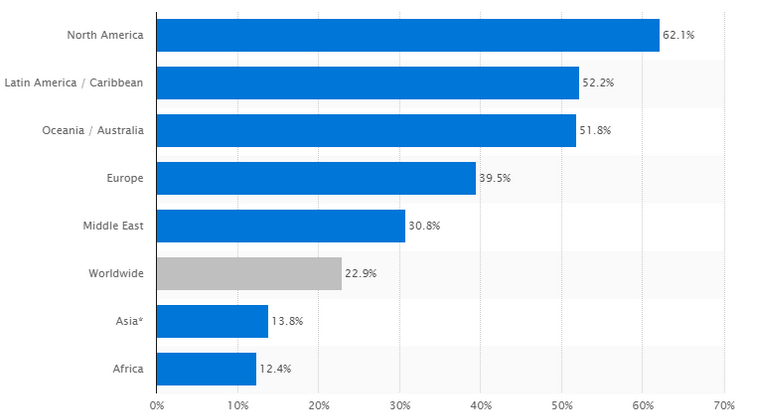
\includegraphics[width=4.00in]{images/sn.png}}
	}
	\caption{Porcentaje de población con perfil en Facebook~\cite{article:FacebookStats} }
	\label{fig:FBStats}
\end{figure}
Esto de por sí no es un dato negativo, el problema viene cuando para
realizar un registro en una página (como por ejemplo, la web de un
diario), la forma más sencilla es conectando con tu perfil personal de
Facebook. Esto causa que, al interaccionar con dicha página (ya sea
publicando un comentario, o cualquier tipo de actividad), te
arriesgues a que aparezca tu nombre real, con todo lo que ello
conlleva. Desde este punto, saber todo acerca de ese usuario es tan
sencillo como buscar en Google su nombre completo y entrar a su perfil
de Facebook, donde aparecen fotos, dirección física, entre otros (por
suerte, esto es algo que desde hace poco podemos
evitar~\cite{article:GDPRGoogle} gracias a la
Ley de Protección de Datos europea, que se adoptará en Mayo de 2018 y respecto a la cual se hará hincapié en este
documento). A todo ello, además, habría que añadir los riesgos
existentes al hacer pública información de corte personal en redes
sociales sin un control adecuado para evitar ataques de \textbf{ingeniería
social} \cite{backstrom2007wherefore,hadnagy2010social}.


En otros casos el iniciar sesión con la cuenta de Google o Facebook
sirve para que dichas empresas conozcan mejor tus gustos y aficiones,
para así ofrecerte publicidad a medida. Si bien esto no es realmente
una invasión a la privacidad por parte del servicio utilizado (excepto
en el caso de que el proveedor no cumple con las normas de uso del
servicio), estamos proporcionando pasivamente de información personal
a terceros, muchas veces desde nuestro desconocimiento, la cual puede
ser utilizada con fines económicos que benefician a la empresa en
cuestión ~\cite{article:compraventa}. De nuevo, esta práctica por sí
sola no vulnera la privacidad a menos que el proveedor de servicio no
cumpla con lo que el usuario aceptó al registrarse en el servicio en
cuestión \cite{diaz2015privacy}. De hecho, es posible una
identificación de un usuario de forma anónima (véase
\url{https://privacypass.github.io/}), sin que ello impida la creación
de perfiles de usuario y el consiguiente despliegue de un sistema de
recomendación.



En definitiva, al igual que en nuestra vida diaria existen peligros a
los que debemos enfrentarnos, como los robos, nuestra actividad en la
red también conlleva varias amenazas, como suplantaciones de identidad
o hurto de información personal. Es más, gran parte de los riesgos en
el ciberespacio son debidos a la compleja proyección entre nuestra
identidad real y la digital (mediante la cual somos aceptados en un
servicio concreto). Dicha proyección es realizada normalmente por un
tercero, al que delegamos la confianza para la correcta gestión de
nuestro \textit{yo} digital, y el riesgo reside en que dicha entidad
no siempre actúa de forma ética.

En el ámbito de la seguridad informática, existe un principio que
trata de impedir la ocurrencia de estas amenazas (entre otras muchas)
y es el \textbf{principio del mínimo
  privilegio}~\cite{schneider2003least}, una piedra angular de la
seguridad que sugiere que toda acción debe ser realizada con los
mínimos privilegios posibles, de forma que cualquier fallo o ataque
tenga el mínimo impacto.

Además, muchas de estas vulneraciones de la privacidad podrían
evitarse en el momento que toda entidad que ofrezca un servicio dejase
claro mediante unas \textbf{normas de uso} cuáles son sus propósitos,
y qué implica que el usuario las acepte (mediante un
\textbf{consentimiento informado}~\cite{lane2014privacy}). Esto,
claro está, también supone la implicación del usuario en preocuparse
sobre qué información personal va a estar expuesta a la hora de
utilizar un servicio \cite{sanchez2018review}.

En este caso, a un proveedor de servicio se le proporciona únicamente la información mínima para la correcta realización del servicio, momento en el cual se le dará consentimiento explícito en caso de estar de acuerdo en utilizar el servicio en cuestión. 

De acuerdo con todo lo anterior, la motivación de este proyecto
responde a la necesidad de dotar al usuario final de recursos para
evaluar y proteger su privacidad. Así, en este proyecto se efectúa un
estudio de diversas tecnologías para proteger la privacidad de un
usuario mediante el anonimato. Además, se estudia un conjunto de
técnicas que pueden suponer una amenaza para nuestra privacidad.
 
Parte de la motivación también reside mi interés en el ámbito de la
seguridad informática. Es un tema de suma importancia (algo que puede
apreciarse en la creciente demanda de expertos en ciberseguridad hoy
en día~\cite{article:expCiberseguridad}) y, por otro lado, sirve para
poner en práctica metodologías y lenguajes estudiados en el grado.

En definitiva, el proyecto abarca un software modular compuesto de
varias herramientas funcionales por sí mismas, donde el
requisito principal es la seguridad del
sistema (\textit{security-by-design}~\cite{paper:secbydesign}) y, sobre
todo, que dicho sistema respete la privacidad del usuario
(\textit{privacy-by-design}~\cite{paper:privacybydesign,cavoukian2009privacy}). Es
más, este requisito pasará a ser
obligatorio a partir de que entre en vigor la GDPR~\cite{article:PbDGDPR}  por
lo que las empresas desarrolladoras de software deberán tener en
cuenta la privacidad de los datos de cada usuario en las fases de
diseño de todos los proyectos.


\lsection{Objetivos y enfoque}

Principalmente se pretenden lograr dos objetivos fundamentales en este
proyecto. El primero es el de hacernos conocedores más a fondo de las
diferentes vías a la hora de anonimizarnos en Internet, las variadas
herramientas que pretenden conseguir este objetivo (así como las que
pretenden identificar a un usuario), como también de las
  diferentes nociones del término
privacidad~\cite{article:danezis2010}. En conclusión, el presente
  proyecto trata realizar una investigación exhaustiva sobre la
dimensión tecnológica privacidad y los caminos para
asegurarla.

Por otro lado, y quizá el objetivo más importante, es el de poner en
práctica los conocimientos adquiridos en la investigación
anteriormente dicha. En este caso se ha diseñado, desarrollado y
probado una herramienta con numerosas y diversas funciones, cuyo
principal propósito es el de proporcionarnos una experiencia
  de navegación en Internet lo más
anónima posible en todo momento.

Por último, aclarar que el presente documento aborda sobre todo la dimensión tecnológica de la privacidad, y no trata el debate legal entre el punto de vista estadounidense ( \textit{privacy-as-secrecy}) y el europeo (\textit{privacy-as-personhood}~\cite{solove2002conceptualizing}). Se trata sobre todo de una investigación a fondo de la privacidad en la red y las diversas maneras de conseguirla.




\lsection{Metodología y plan de trabajo}

Este documento se organiza de la siguiente manera:
\begin{itemize}
	\item Estado  del  Arte: El segundo capítulo explica todos y cada uno de los conceptos de los que trata este proyecto, es decir, el término privacidad, anonimato y la importancia de los mismos hoy en día. Además, se mostrarán ejemplos de herramientas y metodologías para anonimizarse. 
	\item Análisis: El capítulo tres consta de la serie de requisitos, definidos  según  los objetivos  deseados  en  las  aplicaciones  finales  y  delimitados  por  el  alcance  del proyecto.La funcionalidad de la herramienta desarrollada se resume tanto en el catálogo de requisitos como de casos de uso.
	\item Diseño: Este capítulo trata con detalle la fase de diseño, teniendo en cuenta la estructura de la aplicación y el flujo de navegación de la misma 
	\item Desarrollo: En el quinto capítulo se encuentra explicado el método de desarrollo, las librerías utilizadas, los lenguajes en los que está programada la herramienta, las características Software del equipo de desarrollo y el porqué de dicha elección.
	\item Integración, pruebas y resultados: Aquí se tratan las pruebas unitarias realizadas, así como los resultados de las mismas y cómo se han integrado todos los módulos en la aplicación final.
	\item Conclusiones/Trabajo  futuro: Por último, en este capítulo resumimos las conclusiones de la aplicación y el futuro trabajo que se requeriría para que la herramienta continúe creciendo.
\end{itemize}

\newpage \thispagestyle{empty} % Página vacía 